\documentclass{article}

\usepackage{listings}
\usepackage{color}
\usepackage{graphicx}
\usepackage{float}
\usepackage{amsmath}
\usepackage{subfig}
\usepackage{cite}
\usepackage{url}

\begin{document}

\title{Image Analysis - TP3 - Corner detection}

\author{Jander Nascimento, 
\and Raquel Oliveira}

\maketitle

\section{Gradient Images}
	
	\subsection{Horizontal and vertical gradient}

	The gradient is based created based on a vector that points to the highest rate of change in the magnitude. 

\begin{equation}
\bigtriangledown f = \begin{pmatrix}
\frac{\partial f}{\partial x} = M_x\\ 
\frac{\partial f}{\partial y} = M_y
\end{pmatrix}
\label{eq:gradient}
\end{equation}

The gradient can be reached through the Equation \ref{eq:gradient}, but usually (duo to complexity of computation), a filter or linear approximation is used to find a closer result.

There exist several filters that can be used to find the gradient. e.g: sobel and prewitt. Here was used the sobel operator to reach the results.

The sobel operator is a pair of kernels (one for vertical and one horizontal edges detection) which can be convoluted which the image to obtain their respective gradient.

	\begin{figure}[H]
	\centering
	\subfloat[Original Image]{\label{fig:original}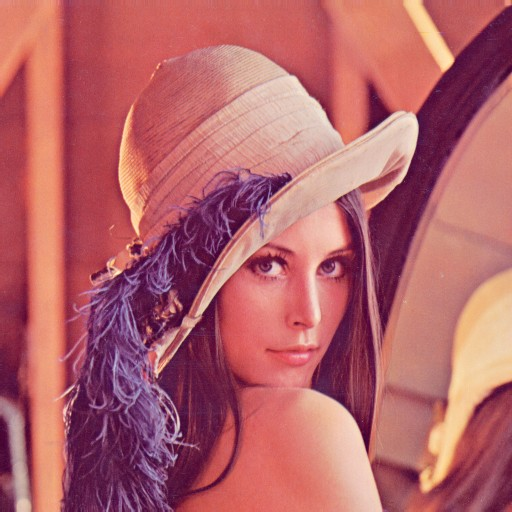
\includegraphics[width=0.3\textwidth]{../lena}}                
	\subfloat[Horizontal Gradient]{\label{fig:horizontal}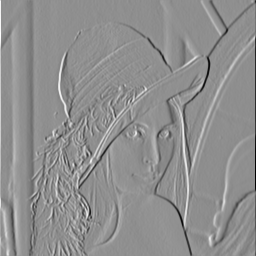
\includegraphics[width=0.3\textwidth]{../img/lena_gradientx}}                
	\subfloat[Vertical Gradient]{\label{fig:vertical}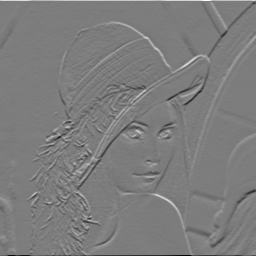
\includegraphics[width=0.3\textwidth]{../img/lena_gradienty}}                
	\caption{Gradient}
	\label{fig:gradient}
	\end{figure}

%\begin{equation}
%magn(\bigtriangledown f) = \sqrt{M_x^{2}+M_y^{2}}\approx \left | M_x \right |+\left | M_y \right |
%\end{equation}

	
	\subsection{Gradient norm}


\section{Corner Detection}




\end{document}


